\documentclass{beamer}
\usetheme{Boadilla}

\newcommand\PRESENTATIONMODE[0]{signal command to allow beamer to work with the header file}



%% Don't import the header multiple times

\ifdefined\HEADERIMPORTED
\else
\newcommand\HEADERIMPORTED[0]{This file is HEADERIMPORTED}
\usepackage{amssymb}

\usepackage{amsmath}
\usepackage[a4paper,includeheadfoot,margin=2.54cm]{geometry}

% For typesetting tree rules
\usepackage{mathpartir}

% For colouring code
\usepackage{xcolor}


\usepackage{array}   % for \newcolumntype macro
\usepackage{tikz-cd}
\usepackage{tabstackengine}
\usepackage{breqn}
\usepackage{stmaryrd}

\usepackage{framed}
\usepackage{listings}

\usepackage{amsthm}
%Theorems
\usepackage[utf8]{inputenc}
\usepackage[english]{babel}
\newtheorem{theorem}{Theorem}[section]
\newtheorem{corollary}{Corollary}[theorem]
\newtheorem{lemma}[theorem]{Lemma}
\newtheorem{property}[theorem]{Property}
\theoremstyle{definition}
\newtheorem{definition}{Definition}[section]

\usepackage{tikz}

\definecolor{grey}{rgb}{0.75, 0.75, 0.75}
\definecolor{DarkGreen}{rgb}{0.1, 0.6, 0.1}

\usetikzlibrary{shapes.geometric,fit}
\usetikzlibrary{arrows,automata,positioning}
\usetikzlibrary{decorations.pathreplacing,calc}



\setstackEOL{\cr}
\setstackgap{L}{\normalbaselineskip}

\newcommand\todo[1]{\textbf{TODO: #1}}
\newcommand\needsRef[1]{\textbf{Reference Needed: (#1)}}
\newcommand\fixLayout[1]{\textbf{Fix Layout: #1}}

\newcommand{\s}{\;}
\newcommand{\doin}[3]{\texttt{do}\s #1 \leftarrow #2 \s\texttt{in}\s #3\s}
\newcommand\apply[2]{#1\s#2}
\newcommand{\pifthenelse}[4]{\texttt{if}_{\textcolor{grey}{#1}}\s#2\s \texttt{then}\s #3 \s\texttt{else} \s#4\s}
\newcommand\ifthenelse[5]{\pifthenelse{#1, #2}{#3}{#4}{#5}}
\newcommand\const[1]{\texttt{C}^{\color{grey} #1}}
\newcommand\return[1]{\texttt{return} \s#1\s}


\newcommand\lam[3]{\lambda #1 \colon {\color{grey}#2}. #3\s}
\renewcommand\u[0]{\texttt{()}}
\newcommand{\U}[0]{\texttt{Unit}}
\renewcommand\t[0]{\texttt{true}}
\newcommand\f[0]{\texttt{false}}
\newcommand{\B}[0]{\texttt{Bool}}
\newcommand{\G}[0]{\Gamma}
\newcommand\D{\Delta}


% draw type relations
\newcommand{\typerelation}[3]{{\color{DarkGreen}#1} \vdash #2 \colon {\color{blue}#3}}
\newcommand\wellformed[2]{{\color{DarkGreen}#1}\vdash {\color{blue}#2}}
\newcommand\wellformedok[2]{\ok{{\color{DarkGreen}#1}\vdash {\color{blue} #2}}}



\newcommand{\gtyperelation}[2]{\typerelation{\G}{#1}{#2}}
 

\newcommand\treerulez[1]{\inferrule{ }{#1}}
\newcommand\treeruleI[2]{\inferrule{#1}{#2}}
\newcommand\treeruleII[3]{\inferrule{#1 \\ #2}{#3}}
\newcommand\treeruleIII[4]{\inferrule{#1 \\ #2 \\ #3}{#4}}
\newcommand\treeruleIV[5]{\inferrule{#1 \\ #2 \\ #3 \\ #4}{#5}}
\newcommand\treeruleV[6]{\inferrule{#1 \\ #2 \\ #3 \\ #4 \\ #5}{#6}}

\newcommand\ntreerulez[2]{(\text{#1})\inferrule{ }{#2}}
\newcommand\ntreeruleI[3]{(\text{#1})\inferrule{#2}{#3}}
\newcommand\ntreeruleII[4]{(\text{#1})\inferrule{#2 \\ #3}{#4}}
\newcommand\ntreeruleIII[5]{(\text{#1})\inferrule{#2 \\ #3 \\ #4}{#5}}
\newcommand\ntreeruleIV[6]{(\text{#1})\inferrule{#2 \\ #3 \\ #4 \\ #5}{#6}}
\newcommand\ntreeruleV[7]{(\text{#1})\inferrule{#2 \\ #3 \\ #4 \\ #5 \\ #6}{#7}}

\newcommand\condtreerulez[3]{(\text{#1})\inferrule{ }{#2}(\text{if } #3)}
\newcommand\condtreeruleI[4]{(\text{#1})\inferrule{#2}{#3}(\text{if } #4)}
\newcommand\condtreeruleII[5]{(\text{#1})\inferrule{#2 \\ #3}{#4}(\text{if } #5)}
\newcommand\condtreeruleIII[6]{(\text{#1})\inferrule{#2 \\ #3 \\ #4}{#5}(\text{if } #6)}
\newcommand\condtreeruleIV[7]{(\text{#1})\inferrule{#2 \\ #3 \\ #4 \\ #5}{#6}(\text{if } #7)}
\newcommand\condtreeruleV[8]{(\text{#1})\inferrule{ #2 \\ #3 \\ #4 \\ #5 \\ #6 }{#7}(\text{if } #8)}



\newcommand{\subtype}[0]{\leq\colon}
\newcommand\subeffect[0]{\leq}

\newcommand{\M}[2]{\texttt{M}_{#1}{#2}}

\newcommand\lamtype[3]{#1 \rightarrow \M{#2}{#3}}
\newcommand{\1}[0]{\texttt{1}}

\newcommand\e[0]{\epsilon}

\newcommand{\db}[1]{{\bf [\![}#1{\bf ]\!]}}
\newcommand{\deno}[1]{\db{#1}}
\newcommand\after\circ
\newcommand\term[1]{\left\langle\right\rangle_{#1}}

\newcommand\bindmu[0]{\mu}
\newcommand\point[1]{\eta_{#1}}
\newcommand\bind[3]{\bindmu_{#1, #2, #3}}

\newcommand\T[2]{T_{#1}{#2}}

\newcommand\pr[2]{\langle#1, #2\rangle}
\newcommand\finpr[2]{\langle #1\rangle_{#2}}

\newcommand\strengtht[0]{\texttt{t}}
% tensor strength Nat-tran
\newcommand\tstrength[3]{\strengtht_{#1, #2, #3}}

% Id morphism
\newcommand\Id[1]{\texttt{Id}_{#1}}

\newcommand\idg[0]{\Id{\G}}
% beta-eta equivalence
\newcommand\beequiv[0]{\approx}
% Substitutions
\newcommand\si{\sigma}

\newcommand{\sub}[1]{\left[#1\right]}
\newcommand{\ssub}[2]{\left[#2 / #1\right]}
\newcommand{\ssi}[0]{\sub{\si}}

% beta-eta equivalence relation
\newcommand{\berelation}[4]{\typerelation{#1}{#2 \beequiv #3}{#4}}
\newcommand{\gberelation}[3]{\gtyperelation{#1 \beequiv #2}{#3}}


% Shortcuts for denotational equality
\newcommand{\denoequality}[4]{\deno{\typerelation{#1}{#2}{#4}} = \deno{\typerelation{#1}{#3}{#4}}}
\newcommand{\gdenoequality}[3]{\denoequality{\G}{#1}{#2}{#3}}

% Shorthand for monad types
\newcommand\mea[0]{\M{\e}{A}}
\newcommand\meb[0]{\M{\e}{B}}
\newcommand\mec[0]{\M{\e}{C}}

\newcommand\tea[0]{\T{\e}{A}}
\newcommand\teb[0]{\T{\e}{B}}
\newcommand\tec[0]{\T{\e}{C}}


\newcommand\moa[0]{\M{\1}{A}}
\newcommand\mob[0]{\M{\1}{B}}
\newcommand\moc[0]{\M{\1}{C}}

\newcommand\toa[0]{\T{\1}{A}}
\newcommand\tob[0]{\T{\1}{B}}
\newcommand\toc[0]{\T{\1}{C}}

\newcommand\aeb[0]{\lamtype{A}{\e}{B}}

% Shorthand for Gammas
\newcommand{\gax}[0]{\G, x\colon A}
\newcommand{\gby}[0]{\G, y\colon B}

% reduction function
\newcommand{\reduce}[0]{reduce}



% Combinators for building delta-based tree proof terms
\newcommand{\deltavrule}[4]{
    \ntreeruleII{Subtype}{\treeruleI{\D}{\typerelation{#1}{#2}{#3}}}{#3 \subtype #4}{\typerelation{#1}{#2}{#4}}}

\newcommand{\deltavruleprime}[4]{
    \ntreeruleII{Subtype}{\treeruleI{\D'}{\typerelation{#1}{#2}{#3}}}{#3 \subtype #4}{\typerelation{#1}{#2}{#4}}}

\newcommand{\deltavruleprimeprime}[4]{
        \ntreeruleII{Subtype}{\treeruleI{\D'}{\typerelation{#1}{#2}{#3}}}{#3 \subtype #4}{\typerelation{#1}{#2}{#4}}}
    
\newcommand{\deltacrule}[6]{
            \ntreeruleII{Subeffect}{\treeruleI{\D}{\typerelation{#1}{#2}{\M{#3}{#4}}}}{\subeffecttree{#3}{#4}{#5}{#6}}{\typerelation{#1}{#2}{\M{#5}{#6}}}}
\newcommand{\deltacruleprime}[6]{
    \ntreeruleII{Subeffect}{\treeruleI{\D'}{\typerelation{#1}{#2}{\M{#3}{#4}}}}{
    \subeffecttree{#3}{#4}{#5}{#6}}{\typerelation{#1}{#2}{\M{#5}{#6}}}}
\newcommand{\deltacruleprimeprime}[6]{
    \ntreeruleII{Subtype}{\treeruleI{\D''}{\typerelation{#1}{#2}{\M{#3}{#4}}}}{
        \subeffecttree{#3}{#4}{#5}{#6}}{\typerelation{#1}{#2}{\M{#5}{#6}}}}
                            

\newcommand{\p}[0]{\pi_1}
\newcommand{\pp}[0]{\pi_2}

% short-hands for weakening
\newcommand{\wrel}[3]{#1 \colon {\color{blue}#2} \triangleright {\color {blue} #3}}
\newcommand{\ok}[1]{{\color{blue} #1} \texttt{ Ok}}
\renewcommand\i[0]{\iota}
\newcommand\w{\omega}
\newcommand\dom[1]{\texttt{dom}(#1)}
\newcommand\x{\times}


\newcommand\fev[1]{fev(#1)}
\newcommand\union[0]{\cup}


% Combinators to build tree proofs
\newcommand{\truleconst}[0]{\ntreeruleI{Const}{\ok{\G}}{\gtyperelation{\const{A}}{A}}}
\newcommand{\truleunit}[0]{\ntreeruleI{Unit}{\ok{\G}}{\typerelation{\G}{\u}{\U}}}
\newcommand{\truletrue}[0]{\ntreeruleI{True}{\ok{\G}}{\typerelation{\G}{\t}{\B}}}
\newcommand{\trulefalse}[0]{\ntreeruleI{False}{\ok{\G}}{\typerelation{\G}{\f}{\B}}}


\newcommand{\E}[0]{\mathbb{E}}
\renewcommand{\dot}{\cdot}
\newcommand{\gens}[0]{\colon\colon=}
\newcommand{\nil}[0]{\diamond}
\newcommand{\ground}[0]{\gamma}

% Terminal object of C
\newcommand{\terminal}[0]{\texttt{\1}}

% The category C
\newcommand{\C}[0]{\mathbb{C}}
\newcommand{\Cz}[0]{\C_0}
\newcommand\DC[0]{\mathbb{D}}

% The category of locally-small categories
\newcommand{\Cat}[0]{\texttt{Cat}}
% Sub-effect Nat-trans
\newcommand{\dse}[2]{\db{#1 \subeffect #2}}

\newcommand\app[0]{\texttt{app}}
\newcommand\cur[1]{\texttt{cur}(#1)}
\newcommand{\ifnt}[1]{\texttt{If}_{#1}}


\newcommand{\setto}{\colon=}
\newcommand{\fv}[1]{\texttt{fv}(#1)}

% shorthand for inserting text to equations
\newcommand\qt[1]{\quad\text{#1}}

% Co-product short-hands
\newcommand\inr[0]{\texttt{inr}}
\newcommand\inl[0]{\texttt{inl}}
    
\newcommand\fld[2]{\left[#1,#2\right]}
\newcommand{\diag}[1]{\delta_{#1}}
\newcommand{\twist}[2]{\tau_{#1, #2}}

\newcommand\ifMorph[3]{\app\after((\fld{\cur{#2\after\pp}}{\cur{#3\after\pp}}\after #1)\times \idg)\after \diag{\G}}


% Polymorphic short-hands
\newcommand\elam[2]{\Lambda #1. #2}
\newcommand{\eapp}[2]{#1\s#2}
\renewcommand{\a}[0]{\alpha}
\newcommand{\all}[2]{\forall #1. #2}
\renewcommand{\P}[0]{\Phi}

\renewcommand{\b}[0]{\beta}
\newcommand{\g}[0]{\gamma}
\renewcommand\d[0]{\delta}
\newcommand\oke[2]{\wellformedok{#1}{#2}}
\newcommand\etyperelation[4]{\typerelation{#1\mid#2}{#3}{#4}}
\newcommand{\gpetyperelation}[2]{\etyperelation{\P}{\G}{#1}{#2}}
\newcommand{\gppetyperelation}[2]{\etyperelation{\P'}{\G}{#1}{#2}}


\newcommand{\eberelation}[5]{\berelation{#1\mid#2}{#3}{#4}{#5}}
\newcommand{\gpeberelation}[3]{\berelation{\P\mid\G}{#1}{#2}{#3}}
\newcommand{\gppeberelation}[3]{\berelation{\P'\mid\G}{#1}{#2}{#3}}

\newcommand{\dotp}[0]{\dot_\P}
\newcommand{\fntype}[2]{#1\rightarrow #2}
\newcommand{\ab}[0]{\fntype{A}{B}}

\newcommand\wrelw[2]{\wrel{\w}{#1}{#2}}
\renewcommand\proof[0]{\paragraph{Proof:}}
\newcommand{\case}[1]{\paragraph{Case #1:}}
\newcommand{\subcase}[1]{\subparagraph{Case: #1}}
\newcommand\bi[0]{By inversion}

%pre-filled effect-weakening relations
\newcommand\ewrel[4]{\wellformed{#1}{\color{black}\wrel{#2}{#3}{#4}}}
\newcommand\pewrel[3]{\ewrel{\P}{#1}{#2}#3}
\newcommand\ppewrel[3]{\ewrel{\P'}{#1}{#2}#3}

\newcommand\subtypep[0]{\subtype_\P}
\newcommand\subtypepp[0]{\subtype_{\P'}}
\newcommand\subeffectp[0]{\subeffect_{\P}}
\newcommand\subeffectpp[0]{\subeffect_{\P'}}
\newcommand\subeffectn[0]{\subeffect_{n}}
\newcommand\subeffectz[0]{\subeffect_{0}}

\newcommand{\allI}[0]{\forall_I}
\newcommand{\allII}[0]{\forall_{I'}}
\newcommand\allIU[0]{\forall_{I\times U}}
\newcommand\type[0]{\texttt{Type}}
\newcommand\effect[0]{\texttt{Effect}}
\newcommand\ciw[0]{\C(I, W)}
\newcommand\ciu[0]{\C(I, U)}
\newcommand\ciuw[0]{\C(I\times U, W)}
\newcommand\cipw[0]{\C(I', W)}
\newcommand\cipu[0]{\C(I', U)}
\newcommand\ciuu[0]{\C(I\times U, U)}
\newcommand\cii[0]{\C(I', I)}
\newcommand\Eff[0]{\texttt{Eff}}
\newcommand\Mul[0]{\texttt{Mul}}
\newcommand\singleton[0]{\ast}
\renewcommand\star[0]{^*}
\renewcommand\bar[1]{\overline{#1}}

\newcommand\subtypeg[0]{\subtype_\g}
\newcommand\subtypepa[0]{\subtype_{\P, \a}}
\newcommand\subtypeppa[0]{\subtype_{\P', \a}}

\newcommand\subtypez[0]{\subtype_{0}}
\newcommand\subtypen[0]{\subtype_{n}}

\usepackage{scalerel,stackengine}
\stackMath
\renewcommand\widehat[1]{%
\savestack{\tmpbox}{\stretchto{%
  \scaleto{%
    \scalerel*[\widthof{\ensuremath{#1}}]{\kern.1pt\mathchar"0362\kern.1pt}%
    {\rule{0ex}{\textheight}}%WIDTH-LIMITED CIRCUMFLEX
  }{\textheight}% 
}{2.4ex}}%
\stackon[-6.9pt]{#1}{\tmpbox}%
}
\parskip 1ex

\newcommand\pstar[0]{\p\star}

\newcommand\edeltavrule[5]{\deltavrule{#1 \mid #2}{#3}{#4}{#5}}

\newcommand\subeffecttreep[4]{\ntreeruleII{Effect}{
    #1\subeffectp #3}{#2 \subtypep #4
}{\M{#1}{
    #2
}\subtypep\M{#3}{#4}}}
\newcommand\subeffecttree[4]{\ntreeruleII{Effect}{
    #1\subeffect #3}{#2 \subtype #4
}{\M{#1}{
    #2
}\subtype\M{#3}{#4}}}


\newcommand{\edeltavruleprime}[5]{
        \deltavruleprime{#1\mid #2}{#3}{#4}{#5}}
    
\newcommand{\edeltavruleprimeprime}[5]{
        \deltavruleprimeprime{#1\mid #2}{#3}{#4}{#5}}
    
\newcommand{\edeltacrule}[6]{
            \ntreeruleII{Subtype}{
                \treeruleI{
                    \D
                }{
                    \typerelation{\P\mid#1}{#2}{\M{#3}{#4}}
                }
            }{
                \ntreeruleII{Effect}{
                    #4 \subtypep #6
                    }{
                         #3 \subeffectp #5
                }{
                    \M{#3}{#4}\subtypep{\M{#5}{#6}}
                }
            }{
                \typerelation{\P\mid #1}{#2}{\M{#5}{#6}}
            }
        }
        

        \newcommand{\edeltacruleprime}[6]{
            \ntreeruleII{Subtype}{
                \treeruleI{
                    \D'
                }{
                    \typerelation{\P\mid #1}{#2}{\M{#3}{#4}}
                }
            }{
                \ntreeruleII{Effect}{
                    #4 \subtypep #6
                }{#3 \subeffectp #5
                }{
                    \M{#3}{#4}\subtypep{\M{#5}{#6}}
                }
            }{
                \typerelation{\P\mid #1}{#2}{\M{#5}{#6}}
            }
        }
                   

        \newcommand{\edeltacruleprimeprime}[6]{
            \ntreeruleII{Subtype}{
                \treeruleI{
                    \D''
                }{
                    \typerelation{\P\mid #1}{#2}{\M{#3}{#4}}
                }
            }{
                \ntreeruleII{Effect}{
                    #4 \subtypep #6
                    }{ #3 \subeffectp #5
                }{
                    \M{#3}{#4}\subtypep{\M{#5}{#6}}
                }
            }{
                \typerelation{\P\mid #1}{#2}{\M{#5}{#6}}
            }
        }

        \newcommand\obj[0]{\texttt{obj }}


        \newcommand{\Tz}[2]{\texttt{T}^0_{#1}#2}
        \newcommand{\Tn}[2]{\texttt{T}^n_{#1}#2}
        \newcommand{\Tm}[2]{\texttt{T}^m_{#1}#2}
        
        \newcommand{\pointz}[1]{\point{#1}^0}
        \newcommand{\pointn}[1]{\point{#1}^n}
        \newcommand{\pointm}[1]{\point{#1}^m}
        
        \newcommand{\bindz}[3]{\bind{#1}{#2}{#3}^0}
        \newcommand{\bindn}[3]{\bind{#1}{#2}{#3}^n}
        \newcommand{\bindm}[3]{\bind{#1}{#2}{#3}^m}
        
        \newcommand\tstrengthz[3]{\tstrength{#1}{#2}{#3}^0}
        \newcommand\tstrengthn[3]{\tstrength{#1}{#2}{#3}^n}
        \newcommand\tstrengthm[3]{\tstrength{#1}{#2}{#3}^m}
        
        \newcommand\set[0]{\texttt{Set}}
        \newcommand\cccat[0]{\textit{CCCat}}

        \newcommand\ev[0]{\vec{\e}}
        \newcommand\emv[0]{\vec{\e_m}}
        \newcommand\env[0]{\vec{\e_n}}
        
        \newcommand\subeffectm[0]{\subeffect_m}
        
        \newcommand\dsem[2]{\db{#1 \subeffectm #2}}
        \newcommand\dsen[2]{\db{#1 \subeffectn #2}}
        \newcommand\dsez[2]{\db{#1 \subeffectz #2}}
        \newcommand\dsep[2]{\db{#1 \subeffectp #2}}
        \newcommand\dsepp[2]{\db{#1 \subeffectpp #2}}
        
        \newcommand\allEn[0]{\forall_{E^n}}
        \newcommand\allEm[0]{\forall_{E^m}}
        
        \newcommand\counit[1]{\boldsymbol{\epsilon}_{#1}}
        \newcommand\unit[1]{\boldsymbol{\eta}_{#1}}
\fi

\title{A Denotational Semantics for Polymorphic Effect Systems}
\subtitle{Part III Project}
\author{Alexander Taylor, at736}
\institute{University of Cambridge}
\date{\today}
\setbeamertemplate{itemize items}[ball]


\begin{document}
\setbeamertemplate{itemize items}[ball]


\input{slides/title}


\begin{frame}[fragile]{Motivating Polymorphic Effect Analysis}    

    \todo{Syntax highlight}
\begin{verbatim}
def logAction(
    action: Unit => String
): Unit {
    log.info(action())
}  
\end{verbatim}

\begin{verbatim}
logAction(() => FireMissiles(); "Launched Missiles)

logAction(() => throwError("My Error"))

logAction(() => readEnvironmentVariables)
\end{verbatim}

    \script{
        - Imagine you're a compiler trying to analyse the side effects of this \texttt{doAction} function here.

        - You're not having the best of times
        - it's used three times with three different side effect - one's irrevocable - you can't speculatively execute it, one alters control flow, and the last accesses immutable state so you can do all sorts of optimisations.
        
        - Using some simple  analysis, you can create three separate instantiations of the function to analyse, so it's not too difficult in this case.
        - However in programs with higher order functions, creating these separate instantiations is undecidable in general

        - With a polymorphic effect system, it becomes a bit easier to analyse programs like this. But how do you know that your tools and optimisations are sound?
    }
\end{frame}

\begin{frame}
    \frametitle{What is Categorical Denotational Semantics?}
    \begin{itemize}
        \setlength\itemsep{3em}
        \item A \textit{compositional} mapping $\deno{-}: \text{Language Structure} \rightarrow \text{Categorical Structure}$
        \item Types and type environments map to objects $\deno{A} \in \obj(\C)$
        \item Well typed terms map to morphisms (arrows) $\deno{\gtyperelation{t}{A}}: \deno{\G} \rightarrow \deno{A}$
        \item Needs to be \textit{sound} $t_1 \beequiv t_2 \implies \deno{t_1} = \deno{t_2}$
        \item And \textit{adequate} $\deno{t_1} = \deno{t_2} \implies t_1 \beequiv t_2$
    \end{itemize}
    

\end{frame}


\begin{frame}
    \frametitle{Contributions}

    \begin{itemize}\setlength\itemsep{3em}
        \item A sound set of requirements for denotational semantics of effect-polymorphic languages.
        \item A method to construct models for effect-polymorphic languages in $\set$.
        \item A proof of adequacy of such a model.
    \end{itemize}

    \script{
        - There are three main contributions here
            - A set of requirements to make a sound model of an effect polymorphic language
            - A construction of models for polymorphic languages in the category of Sets
            - And for a particular language I've proved adequacy.
    }
\end{frame}


\begin{frame}{Language features (2.B) - Graded Monads}
    A (strong) graded monad consists of:
        \begin{itemize}
            \setlength\itemsep{3em}
            \item An indexed functor $\T{\e}{}: \C\rightarrow \C$
            \item Indexed Join and Unit natural transformations
            \begin{itemize}
                \item  $\bind{\e_1}{\e_2}{A}: \T{\e_1}{\T{\e_2}{A}}\rightarrow \T{\e_1\dot \e_2}{A}$\
                \item $\point{A}: A\rightarrow \T{\1}{A}$
            \end{itemize}
            \item Tensor strength natural transformation $\tstrength{\e}{A}{B}: A\times\T{\e}{B}\rightarrow \T{\e}{(A\times B)}$
        \end{itemize}

        \script{
            - A solution is a graded monad.
            - We now have one functor, indexed by a monoid of effect symbols. The rules and morphisms stay the same but are now also indexed. 

        }    
\end{frame}


\begin{frame}{An Effectful Language}
    \begin{align*}
        v ::= & \const{A} \mid x\mid \t \mid\f \mid\u\mid\lam{x}{A}{v}\mid\apply{v_1}{v_2}\mid\return{v}\\
        & \mid\doin{x}{v_1}{v_2}\mid\pifthenelse{A}{v}{v_1}{v_2} 
    \end{align*}
    
    \begin{align*}
        A, B, C ::= \g\mid \ab \mid\mea
    \end{align*}

    \[
        \ntreeruleI{Return}{\gtyperelation{v}{A}}{\gtyperelation{\return{v}}{\moa}}
    \quad
    \ntreeruleII{Apply}{\gtyperelation{v_1}{\ab}}{\gtyperelation{v_2}{A}}{\gtyperelation{\apply{v_1}{v_2}}{B}}
    \]

    \script{
        - Let's now describe a simple effectful, lambda-calculus-based, language, EC.
        - It has an explicit graded monad, subtyping, if-statements
    }
\end{frame}


\begin{frame}{An Effectful Language}
    \begin{align*}
        v ::= & \put^{\M{\1}{Unit}} \mid x\mid \t \mid\f \mid\u\mid\lam{x}{A}{v}\mid\apply{v_1}{v_2}\mid\return{v}\\
        & \mid\doin{x}{v_1}{v_2}\mid\pifthenelse{A}{v}{v_1}{v_2} 
    \end{align*}
    
    \begin{align*}
        A, B, C ::= \B \mid \U \mid \ab \mid\mna
    \end{align*}

    \[
        \ntreeruleI{Return}{\gtyperelation{v}{A}}{\gtyperelation{\return{v}}{\M{0}{A}}}
    \quad
    \ntreeruleII{Apply}{\gtyperelation{v_1}{\ab}}{\gtyperelation{v_2}{A}}{\gtyperelation{\apply{v_1}{v_2}}{B}}
    \]

    \[
    \M{n}{A} \subtype \M{n+1}{A}    
    \]

    \script{
        - Let's now describe a simple effectful, lambda-calculus-based, language, EC.
        - It has an explicit graded monad, subtyping, if-statements
    }
\end{frame}



\begin{frame}{Semantics of EC}
    \begin{itemize}
        \setlength\itemsep{3em}
        \item Can build a model of EC when we have
        \begin{itemize}
            \item CCC
            \item Strong Graded Monad
            \item Co-product and Subtyping (morphisms for if-statements)
        \end{itemize}
        \item We'll call this an S-category
    \end{itemize}
    
    \[
        \scalebox{.8}{$
        \ntreeruleI{Return}{f = \deno{\gtyperelation{v}{A}}}{\deno{\gtyperelation{\return{v}}{\moa}} = \point{A} \after f}
        \quad
        \ntreeruleI{Fn}{f = \deno{\typerelation{\gax}{v}{B}} : \G \times A \rightarrow B}{\deno{\gtyperelation{\lam{x}{A}{v}}{\ab}} = \cur{f} : \G \rightarrow B^A}
        $}
    \]

    \script{
        - As described, all of the language features can be modelled in a cartesian closed category with a graded monad, a coproduct, and subtyping morphisms.

        - Known as an S-Category

        - Here's an example, if we have the denotation of an expression here, we can get the denotation of using it as a pure computation by postcomposing with the unit of the graded monad.

    }
\end{frame}


\begin{frame}{Semantics of EC}
    \begin{itemize}
        \setlength\itemsep{3em}
        \item Can build a model of EC with sets and functions
        \item Types map to sets   
        \begin{itemize}
            \item $\deno{\u} = \{\singleton\}$, $\deno{\B} =  \{ \top, \bot \}$
            \item $\deno{\ab} = \deno{A} \implies \deno{B}$
            \item $\deno{\M{n}{A}} = \setcomp{(n', a)}{a\in \deno{A}, n' \leq n}$
        \end{itemize}
        \item Well typed terms map to functions \begin{itemize}
            \item $\deno{\gtyperelation{\t}{\B}} = \rho \mapsto \top$
            \item $\deno{\gtyperelation{\put}{\M{\1}{\U}}} = \rho \mapsto (1, \singleton)$
            \item $\begin{aligned}
                \deno{\gtyperelation{\doin{x}{v_1}{v_2}}} & = \rho \mapsto  \\
                & \text{let } (n', a) = \deno{\gtyperelation{v_1}{\mna}}(\rho) \\
                & \text{ and }(m', b) = \deno{\typerelation{\gax}{v_2}{\mmb}})(\rho, a) \\
                & \text{ in } (m' + n', b)
            \end{aligned}$
        \end{itemize}
    \end{itemize}


    \script{
        - As described, all of the language features can be modelled in a cartesian closed category with a graded monad, a coproduct, and subtyping morphisms.

        - Known as an S-Category

        - Here's an example, if we have the denotation of an expression here, we can get the denotation of using it as a pure computation by postcomposing with the unit of the graded monad.

    }
\end{frame}

\todo{needs to be indexed by n instead}

\begin{frame}[fragile]{An Ugly Example}
\todo{syntax highlight this}
    \begin{lstlisting}[
        mathescape,
        columns=fullflexible,
        basicstyle=\fontfamily{lmvtt}\selectfont,
      ]
let $twiceIO$ = $\lambda$ $action$: $\M{\texttt{IO}}{\U}$. (
    do $\_$ $\texttt{<-}$ $action$ in $action$
)

let $twiceState$ = $\lambda$ $action$: $\M{\texttt{State}}{\U}$. (
    do $\_$ $\texttt{<-}$ $action$ in $action$
)

do $\_$ $\texttt{<-}$ $twiceState$(increment) in $twiceIO$(writeLog)
    \end{lstlisting}
    \script{
        - Here's a program that's quite ugly with lots of code reuse, since we explicitly state types in the expressions. 
        - we end up with two instantiations of the same function - more work for the compiler
    }
\end{frame}



\begin{frame}{Let's Add Polymorphism}
   
    \begin{align*}
        v::=\text{..}\mid\elam{\a}{v}\mid\eapp{v}{\e}
    \end{align*}
    
    \begin{align*}
        A, B, C::=\text{...}\mid \all{\a}{A}
    \end{align*}
    
    \begin{align*}
        \e ::= e \mid \a \mid \e\dot\e
    \end{align*}
    
        \[
            \ntreeruleI{Effect-Gen}{\etyperelation{\P,\a}{\G}{v}{A}}{\gpetyperelation{\elam{\a}{v}}{\all{\a}{A}}}
            \quad
            \ntreeruleII{Effect-Spec}{\gpetyperelation{v}{\all{\a}A}}{\wellformed{\P}{\e}}{\gpetyperelation{\eapp{v}{\e}}{A\ssub{\a}{\e}}}    
        \]
        \script{
            - Let's now add some polymorphism syntax to EC.
            - This gives us the polymorphic effect calculus.
            - Notice now that in our type rules, we now have an effect-variable environment. Important later
        }
    \end{frame}
    

\input{slides/uglyExampleWithPolymorphism}


\begin{frame}{How do we Model the Semantics of a Polymorphic Language?}

    \begin{itemize}
        \setlength\itemsep{3em}
        \item For a fixed effect variable environment $\P$ and terms with no polymorphic sub-terms, we have EC
        \item Effect-variable environments of length $n$ are isomorphic by $\a$-equivalence
    \end{itemize}
    
    

    \script{
        - If we fix the effect-variable environment, and disallow polymorphic terms, then PEC terms become EC terms for a particular instantiation.
        - We already know how to build models for PEC
        -It's also the case that effect-variable environments can type the same set of relations, upto alpha equivalence.
        - So there is a countable set of these EC instantiations
    }
\end{frame}

\begin{frame}{How do we Model the Semantics of a Polymorphic Language?}

\begin{minipage}{0.45\linewidth}
    \begin{itemize}
        \item So we instantiate an S-category for each environment.
        \item The type rule for quantification requires us to move between categories \todo{Type rule here}.
        \item Functors are required.
    \end{itemize}
\end{minipage}\quad \begin{minipage}{0.45\linewidth}
    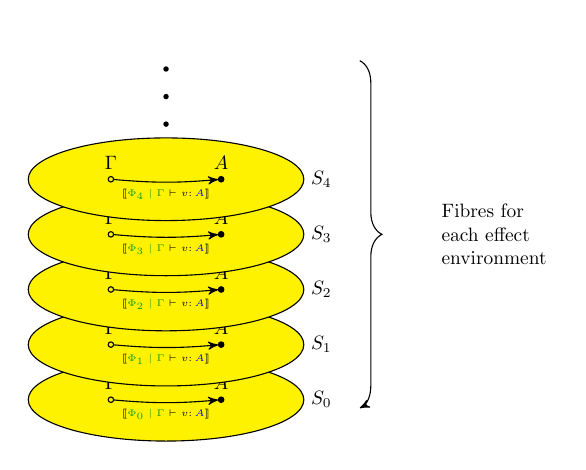
\begin{tikzpicture}[->,>=stealth', scale=0.7, every node/.style={scale=0.7}]
        %draw the s-category stack
\foreach \y[count=\c,evaluate={\yi=int(\c-1)}] in {2, 3, 4, 5, 6}{
    \node[ellipse, draw,fill=yellow, fill opacity=1, minimum width=5cm, minimum height=15mm,label=right:$S_\yi$] (s\yi) at (8,\y){};
    \node[circle, draw, inner sep=1pt, label=above:{$\G$}] (g\yi) at (7,\y){};
    \node[circle, draw, inner sep=1pt, fill, label=above:{$A$}] (a\yi) at (9,\y){};
    \draw[->](g\yi) to[bend right=5] node[below]{\tiny $\deno{\etyperelation{\P_\yi}{\G}{v}{A}}$} (a\yi);
}

% Hidden ellipse to draw functors to
\node[ellipse, minimum width=5cm, minimum height=15mm] (s5) at (8,8){};

%Draw the ... for the s-category stack
\foreach \y[count=\c,evaluate={\yi=int(\c-1)}] in {7, 7.5, 8}{
    \node[fill, circle, inner sep=1pt] (p\yi) at (8, \y){};
}

% draw the re-indexing functors


%Draw the bracket

\draw [decoration={brace,amplitude=8pt},decorate] ($(s5)+(10em,1ex)$) -- ($(s0)+(10em,-1ex)$);
\node[text width=20mm] (Label) at (14,5){Fibres for each effect environment};
\end{tikzpicture}

\end{minipage}

\script{
    - So we can imagine a stack of these S-Categories, called fibres
    - In order to model polymorphism, we need to have ways of moving morphisms between these fibres - we need functors
}
\end{frame}

% 
\begin{frame}{Base Category}
\begin{itemize}
    \item Need to be able to reason about the effect environment categorically
    \item Model effects and their environments using category $\Eff$: \begin{itemize}
        \item Objects are products of the set of ground effects $\{\singleton\} , E, E\times E,... E^n..$
        \item Morphisms are monotone functions
    \end{itemize}
    \item Represent $\P$ as an object $E^n$
    \item Transformations (e.g. substitutions) between environments become functions
\end{itemize}

\script{
    - So we need a way of reasoning about the transformations of effect-variable environments in a category theoretic manner
    - To do this, we need a base category, containing a terminal object, an object $U$ representing the kind of effects, and finite products on $U$ 
    - $U^n$ represents the effect-variable environment of length $n$. We'll now use $I$ to indicate this.
    
    - Since all the ground effects have morphisms in this category, we can construct morphisms for substitutions and weakenings of the effect environment.
}
\end{frame}



\begin{frame}{Indexed Category}

    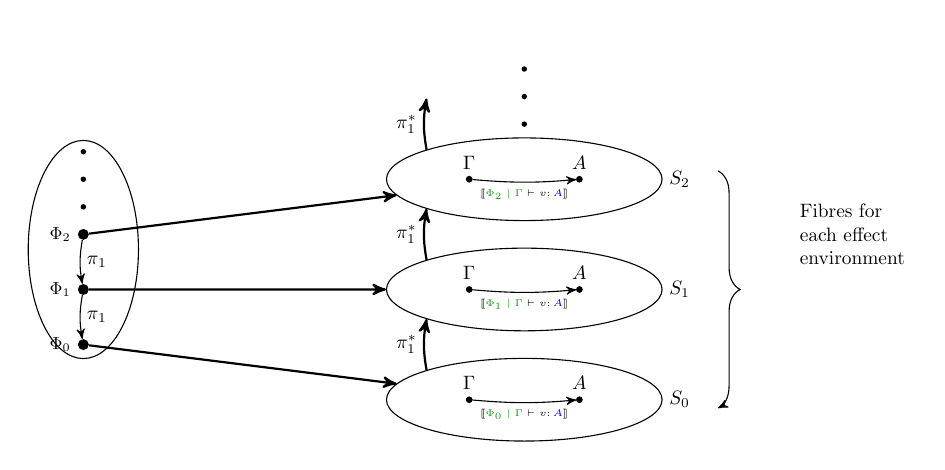
\begin{tikzpicture}[->,>=stealth', scale=0.7, every node/.style={scale=0.7}]
        % Draw the env objects
        \foreach \y[count=\c,evaluate={\yi=int(\c-1)}] in {3, 4, 5}{
            \node[fill,circle,inner sep=2pt,label=left:{\small $\P_\yi$}] (d\yi) at (0,\y) {};
        }

        % draw the ... above the env objects
        \foreach \y[count=\c,evaluate={\yi=int(\c-1)}] in {5.5, 6, 6.5}{
            \node[fill, circle, inner sep=1pt] (dd\yi) at (0,\y){};
        }
        % Draw the index category
        \node[fit=(d0) (d1) (d2) (dd0) (dd1) (dd2),ellipse,draw,minimum width=2cm] {};

        %draw the s-category stack
        \foreach \y[count=\c,evaluate={\yi=int(\c-1)}] in {2, 4, 6}{
            \node[circle, draw, inner sep=1pt, fill, label=above:{$\G$}] (g\yi) at (7,\y){};
            \node[circle, draw, inner sep=1pt, fill, label=above:{$A$}] (a\yi) at (9,\y){};
            \draw[->](g\yi) to[bend right=5] node[below]{\tiny $\deno{\etyperelation{\P_\yi}{\G}{v}{A}}$} (a\yi);
            \node[ellipse, draw, minimum width=5cm, minimum height=15mm,label=right:$S_\yi$] (s\yi) at (8,\y){};
        }

        % Hidden ellipse to draw functors to
        \node[ellipse, minimum width=5cm, minimum height=15mm] (s3) at (8,8){};

        %Draw the ... for the s-category stack
        \foreach \y[count=\c,evaluate={\yi=int(\c-1)}] in {7, 7.5, 8}{
            \node[fill, circle, inner sep=1pt] (p\yi) at (8, \y){};
        }

        % Draw index arrows
        \foreach \i in {0, 1, 2}{
            \draw[->, thick] (d\i) to (s\i);
        }

        % draw the re-indexing functors

        \foreach \source[count=\dest] in {0, 1, 2}{
            \draw[->, thick](s\source.north west) to[bend left=10] node[left]{$\pstar$} (s\dest.south west);
        }

        % Draw the quantification functors
        %\foreach \dest[count=\source] in {0, 1, 2}{
        %    \draw[->, thick] 
        %    (s\source.south east) to[bend left=10] node[right]{$\forall_{\P_\dest}$} (s\dest.north east);
        %}

        % Draw the internal morphisms in base category
        \foreach \dest[count=\source] in {0, 1}{
            \draw[->]
            (d\source) to[bend right=10] node[right]{$\p$} (d\dest);
        }

        %Draw the bracket

        \draw [decoration={brace,amplitude=8pt},decorate] ($(s2)+(10em,1ex)$) -- ($(s0)+(10em,-1ex)$);
        \node[text width=20mm] (Label) at (14,5){Fibres for each effect environment};
    \end{tikzpicture}


    \script{
        - So now we can construct this structure
        - called an index category
        - We have a functor mapping each object representing an effect-variable environment to the relevant S-category fibre.
        - Also contravariantly, meaning the direction of the morphism changes, maps morphisms in the base category to re-indexing functors between the relevant fibres.
        - So now we can perform substitutions and weakenings on the effect environment and get the right behaviour on the semantics of the EC instantiation
    }
    
\end{frame}


% 
\begin{frame}{Quantification}
    \begin{itemize}\setlength\itemsep{2em}
        \item What about effect-generalisation?
        \item $\ntreeruleI{Effect-Gen}{\etyperelation{\P,\a}{\G}{v}{A}}{\etyperelation{\P}{\G}{\elam{\a}{v}}{\all{\a}{A}}}$
        \item Need to map $\deno{\etyperelation{\P,\a}{\G}{v}{A}}$ to $\deno{\etyperelation{\P}{\G}{\elam{\a}{v}}{\all{\a}{A}}}$
        \item For specialisation to work, needs: $\pstar\dashv\allI$
    \end{itemize}


    
    \script{
        - We now need to think about the polymorphic terms
        - For quantification, we need another functor, $\allI$ which maps a type rule with an extra effect variable to one quantified over that variable
        - In order for specialisation to work, this quantification functor needs to be a right adjoint to the opposite operation of weakening the effect environment
        - Adjunction of functors is essentially a weaker version of an isomorphism of the categories they're between.
        - Going out on one functor and coming back on the other isn't quite the same as the identity, but it has a well defined action.
    }

\end{frame}


    
\begin{frame}{Instantiating a Model (1)}

        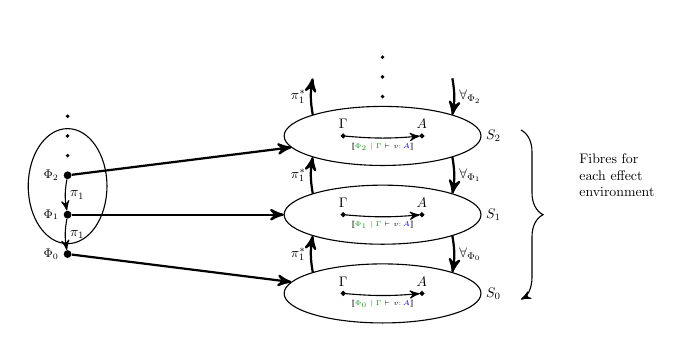
\begin{tikzpicture}[->,>=stealth', scale=0.5, every node/.style={scale=0.5}]
            % Draw the env objects
            \foreach \y[count=\c,evaluate={\yi=int(\c-1)}] in {3, 4, 5}{
                \node[fill,circle,inner sep=2pt,label=left:{\small $\P_\yi$}] (d\yi) at (0,\y) {};
            }
    
            % draw the ... above the env objects
            \foreach \y[count=\c,evaluate={\yi=int(\c-1)}] in {5.5, 6, 6.5}{
                \node[fill, circle, inner sep=1pt] (dd\yi) at (0,\y){};
            }
            % Draw the index category
            \node[fit=(d0) (d1) (d2) (dd0) (dd1) (dd2),ellipse,draw,minimum width=2cm] {};
    
            %draw the s-category stack
            \foreach \y[count=\c,evaluate={\yi=int(\c-1)}] in {2, 4, 6}{
                \node[circle, draw, inner sep=1pt, fill, label=above:{$\G$}] (g\yi) at (7,\y){};
                \node[circle, draw, inner sep=1pt, fill, label=above:{$A$}] (a\yi) at (9,\y){};
                \draw[->](g\yi) to[bend right=5] node[below]{\tiny $\deno{\etyperelation{\P_\yi}{\G}{v}{A}}$} (a\yi);
                \node[ellipse, draw, minimum width=5cm, minimum height=15mm,label=right:$S_\yi$] (s\yi) at (8,\y){};
            }
    
            % Hidden ellipse to draw functors to
            \node[ellipse, minimum width=5cm, minimum height=15mm] (s3) at (8,8){};
    
            %Draw the ... for the s-category stack
            \foreach \y[count=\c,evaluate={\yi=int(\c-1)}] in {7, 7.5, 8}{
                \node[fill, circle, inner sep=1pt] (p\yi) at (8, \y){};
            }
    
            % Draw index arrows
            \foreach \i in {0, 1, 2}{
                \draw[->, thick] (d\i) to (s\i);
            }
    
            % draw the re-indexing functors
    
            \foreach \source[count=\dest] in {0, 1, 2}{
                \draw[->, thick](s\source.north west) to[bend left=10] node[left]{$\pstar$} (s\dest.south west);
            }
    
            % Draw the quantification functors
            \foreach \dest[count=\source] in {0, 1, 2}{
                \draw[->, thick] 
                (s\source.south east) to[bend left=10] node[right]{$\forall_{\P_\dest}$} (s\dest.north east);
            }
    
            % Draw the internal morphisms in base category
            \foreach \dest[count=\source] in {0, 1}{
                \draw[->]
                (d\source) to[bend right=10] node[right]{$\p$} (d\dest);
            }
    
            %Draw the bracket
    
            \draw [decoration={brace,amplitude=8pt},decorate] ($(s2)+(10em,1ex)$) -- ($(s0)+(10em,-1ex)$);
            \node[text width=20mm] (Label) at (14,5){Fibres for each effect environment};
        \end{tikzpicture}

    \begin{itemize}
        \item Can we actually instantiate a category with the required structure? 
        \item Starting point: a model of EC in $\set$
    \end{itemize}
    
    \script{
        - So far, we've only said what structures are required to model PEC.
        - Haven't shown that there actually exists an indexed category with the required properties
        - so let's do that
        - It's fairly well known that you can instantiate models of languages with the same features as EC in the category of sets and functions
        - We want to extend one of these models into one for PEC
    }
\end{frame}

\begin{frame}{Instantiating a Model (2) - Fibres}
    \begin{itemize}\setlength\itemsep{3em}
        \item The fibre $\C(n)$ is the category of functors $[E^n, \set]$
        \item I.E. objects are functions that take a vector of ground effects and return a set $\deno{\wellformedt{\P}{A}}: E^n \rightarrow \obj(\set)$.
        \item Morphisms are dependent functions that return functions in $f: (\ev: E^n)\rightarrow A\ev\rightarrow B\ev$
        \item These fibres have S-Category features
    \end{itemize}

    \script{
        - Now we can think about the fibres
        - These are functor categories
        - I.E. their objects are functions returning sets and their morphisms are dependently typed functions
        - We can construct all the of the S-Category structure  as pointwise
    }
\end{frame}

\begin{frame}{Instantiating a Model (4) - Functors and Adjunctions}
\begin{itemize}
    \item Re-indexing functors act by pre-composition
    \begin{align*}
        A\in&\quad [E^n, \set]\\
        \theta\star(A) \emv =&\quad  A(\theta(\emv))\\
        \theta\star(f) \emv =&\quad f(\theta(\emv)): \theta\star(A) \rightarrow \theta\star(B)\\
    \end{align*}
    \item The quantification functor takes a product over all ground effects
    \begin{align*}
        \allEn(A)\env =&\Pi_{\e\in E}{A(\env, \e)}
    \end{align*}
\end{itemize}
    


    

    \script{
        - Finally, we need to construct the various functors
        - Reindexing functors are done using precomposition
        - quantification consists of a product over all ground effects
    }
\end{frame}


\begin{frame}{The End}
    \begin{itemize}\setlength\itemsep{3em}
        \item Sound: Proved for all indexed S-Categories \checkmark
        \item Compositional: By the definition of denotations \checkmark
        \item Adequate: Proved for an instantiation in $\set$ \checkmark
    \end{itemize}

    \textbf{Dissertation: } \texttt{https://github.com/Al153/Part3Project/tree/master/diss}

    \script{Thanks}
    
\end{frame}



\end{document}